\subsection{Pure \ch{NO} measurements with synthetic air}
\label{sec:no}

After confirming that our generator produced a clean Ozone stream, we
turned towards the question whether it is possible to actually measure
\ch{NO} or not. Furthermore we wanted to reach an experimental
estimate for the necessary reaction pathlength as computed in
Section~\ref{sec:requirements} (c.\,f.\
Tab.~\ref{tab:pathlength}). 

\subsubsection{Setup}
\label{sec:no-setup}

To be able to measure the Nitrogen
Monoxide concentration directly without additional corrections, we had
to make sure that the used sample air was Nitrogen Dioxide free. This
lead us to the setup depicted in Figure~\ref{fig:no-setup}. We used
synthetic air and \ch{NO} calibration gas with a known \ch{NO} concentration ($c
= \SI{8.177}{ppb}$) together with a mass flow controller to generate
precisely controlled sample air. To minimize the influence on the
pressure inside the cavity, we decided to overflow the air input
instead of bypassing the cavity pump as is done during Helium
calibration. Thus we set the synthetic air flow to $\Phi_{\text{air}}$
to \SI{3}{\liter\per\minute}. The cavity itself was in the standard
setup described in Section~\ref{sec:inclusion}, except for the
reaction pathlength whch was varied between \SI{5}{\meter},
\SI{10}{\meter} and \SI{15}{\meter}. For each of these lengths we
varied the \ch{NO} calibration gas flow between \num{0} and
\SI{0.03}{\liter\per\minute}. As zeror air we used ambient lab air
together with a zero air cartridge.

\begin{figure}[htbp]
  \centering
  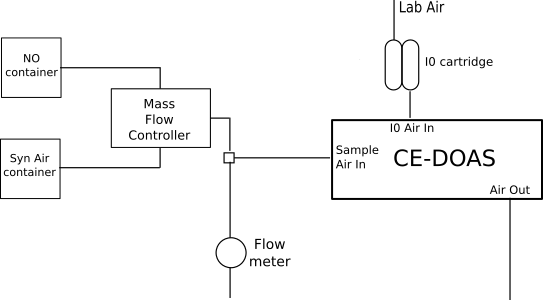
\includegraphics[width=0.6\textwidth]{no_setup.png}
  \caption{Setup of the calibration measurement}
  \label{fig:no-setup}
\end{figure}

In order be able to compare the measured \ch{NO} concentration to the
actual concentration in the air stream, we have to convert the applied
\ch{NO} flow to a concentration, too. We can do this using the
following formula
\begin{align}
  c_{\ch{NO}} = c \cdot \frac{\Phi_{\ch{NO}}}{\Phi_{\text{air}} +
  \Phi_{\ch{NO}}}. \label{eq:c-flow}
\end{align}

\subsubsection{Results}
\label{sec:no-results}

Figure~\ref{fig:ts} shows the timeseries of the \ch{NO} and \ch{O3}
concentration. Each of the three clusters corresponds from left to
right to the reaction path length of \num{5}, \num{10} and
\SI{15}{\meter}. Turning first towards the Ozone concentration on the
right hand side, we see that its concentration is constant within its
error margins. These, however, are large. This is to be expected, as
the absorption cross section of \ch{O3} in the visual spectrum is weak
compared to the cross section of \ch{NO2}. If now the \ch{NO2} signal
becomes strong the fitting of the weaker \ch{O3} absorption becomes
harder and leads to larger errors. Nevertheless, the Ozone level seems
acceptably stable, which indicates that not to many Ozone destroying
reactions took place. This is again what we expected in this very pure
sample air which should only allow for the oxidation of
\ch{NO}. Lastly the shape of the Ozone timeseries does not seem to
depend on the reaction pathlength.

Looking at the \ch{NO} timeseries on the right hand side of
Figure~\ref{fig:ts} we see that the overall shape of three
measurements are similar. For the reaction pathlength of $l=
\SI{5}{\meter}$ we see slight deviations. The rising flanks take
longer to reach a stable plateau than during the other two
measurements. Furthermore the first three plateaus are not visible,
however, the reason for this lies in the fact that they were
skipped. This behaviour indicates that the reaction
pathlength is not long enough for the whole conversion from \ch{NO} to
\ch{NO2} to take place in the tube. As we know we have more than
\SI{1}{ppm} (the figure indicates around \SI{2}{ppb}) Ozone mixed with
the sample air. This amount is enough to oxidize the Nitrogen Monoxide
completely given time. If the time in the reaction tube is too short,
some of the \ch{NO} will not be converted and therefore react with the
Ozone in the cavity itself. With that there are two sources and one
sink of \ch{NO2} in the cavity. The cavity entrance and the reaction
taking place within the cavity as source and the cavity drain as
sink. This system should stabilize at an equilibrium which should be
close to the state where all \ch{NO} is converted, as the dwell time
in the cavity should be long enough for the complete conversion even
taking into account the bad mixing behaviour within. If we know look
at two scenarios: One where at the beginning the cavity is \ch{NO2}
free and one where at the beginning the cavity contains more \ch{NO2}
than at the stable equilibrium. In the first case the main mechanism
to raise the \ch{NO2} concentration to the equilibrium level is by the
`reaction source', which is rather slow, because of the mixing
behaviour. In the second scenario we have more \ch{NO2} to begin with,
so the input flow together with the reaction in the cavity can not
keep up the level. So the excess concentration will be depleted by the
cavity drain, which is a constant time and rather fast process. These
two scenarios are prototypical for the rising and the falling flanks
respectively and thus explain, why we see the slow flanks rising,
while there seems to be no effect on the falling side.

\begin{figure}[htbp]
  \centering
  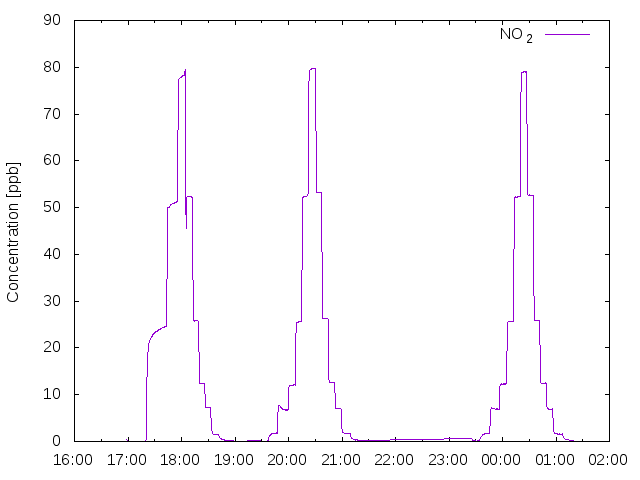
\includegraphics[width=0.45\textwidth]{20160222_NO_fixI0_NO_ts.png}
  \hfill
  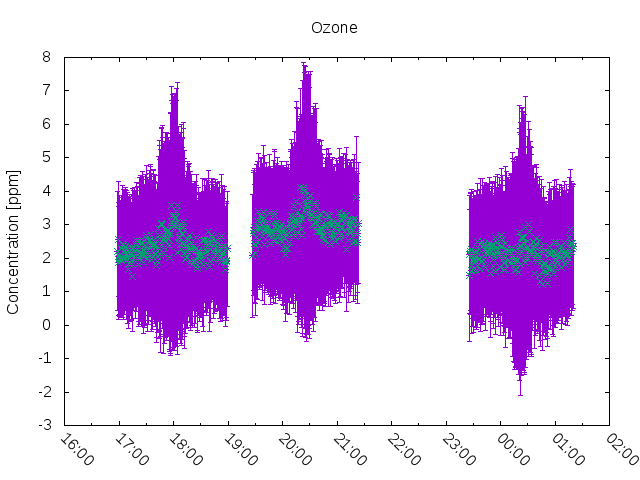
\includegraphics[width=0.45\textwidth]{20160222_NO_fixI0_O3_ts.png}
  \caption{Timeseries of the \ch{NO} and \ch{O3} concentration. The
    three clusters correspond to the three used reaction pathlengths
    $l = 5, 10$ and \SI{15}{\meter}.}
  \label{fig:ts}
\end{figure}
\todo{Redo figures with sensible dimensions}

Comparing next the \ch{NO2} plateaus between multiple pathlengths, we
see that the concentrations seem to coincide. Averaging them and
plotting them over the pathlength we yield Figure~\ref{fig:no-length},
which confirms this assertion. The data points at coresponding flows
were linearly interpolated to make drifts more tangible. The fits are
also plotted in the figure. The interpolation showed that the slope
was undiscernible from zero in each case. At the \SI{5}{\meter}
setting one of the red and one of the violet data points seem to be
off. These two data points correspond to the rising flank discussed
extensively above. It seems that at these two data points the
equilibrium had not been reached and we averaged to early.

\begin{figure}[htbp]
  \centering
  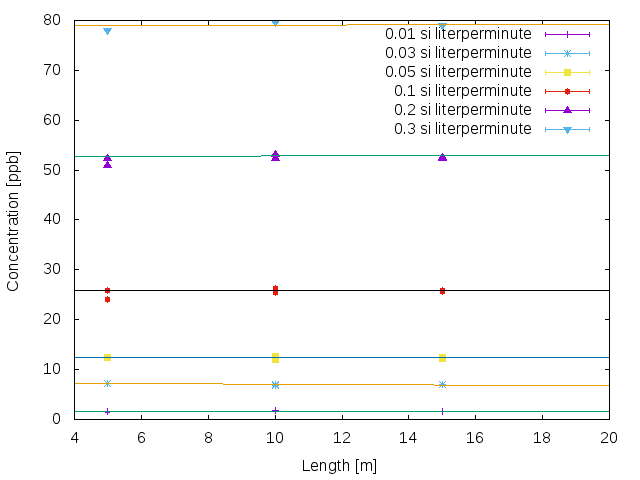
\includegraphics[width=0.7\textwidth]{20160222_NO_fixI0_NO_length.png}
  \caption{\ch{NO} concentration dependence on reaction path
    length. The data points are colored depending on the applied
    \ch{NO} flow. All data points were linearly interpolated. The
    results can also be found in the plot.}
  \label{fig:no-length}
\end{figure}

Since Figure~\ref{fig:no-length} indicated that the measured
concentrations aret pathlength independent (except for two outliers),
we can use all of them to research the correlation between our
measured concentrations and the ones computed from the flow by
Equation~\eqref{eq:c-flow}. The result can be seen in
Figure~\ref{fig:no-calib} together with a linear regression. The
regression formula yields

\begin{align*}
  y = 0.994 \cdot x -0.00234.
\end{align*}
\todo{add uncertainties}

Thus we see that the deviation between the measured and computed
concentration lies in the per mill regime. We see that under these
controlled conditions our converter works and does not introduce
tangible systematic errors. Figure~\ref{fig:ts} implies that a
\SI{10}{\meter} reaction path is sufficient and will therefore used
for the following experiments.

\begin{figure}[htbp]
  \centering
  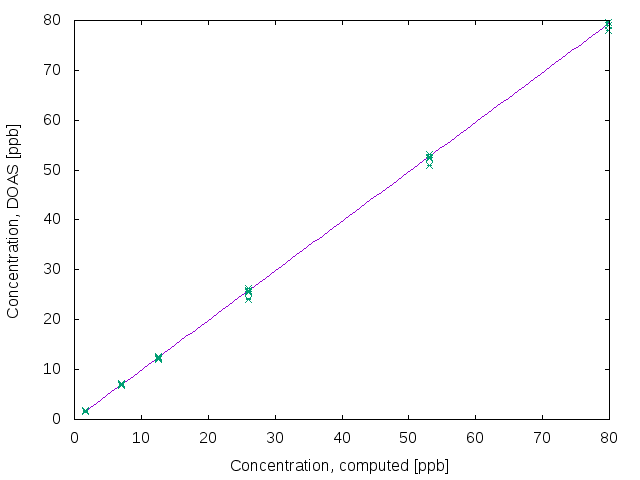
\includegraphics[width=0.7\textwidth]{20160222_NO_fixI0.png}
  \caption{Correlation plot of the computed and the measured \ch{pNO}
    concentration.}
  \label{fig:no-calib}
\end{figure}

%%% Local Variables:
%%% mode: latex
%%% TeX-master: "../Bachelor"
%%% End:
